\documentclass[a4paper,12pt]{article}
\usepackage{graphicx}
\graphicspath{ {../images/} }
\usepackage{hyperref}
\hypersetup{
    colorlinks=true,
    linkcolor=blue,
    filecolor=magenta,      
    urlcolor=blue,
}
 
\urlstyle{same}

\newcommand{\tab}[1]{\hspace{.1\textwidth}\rlap{#1}}

\begin{document}
	
\begin{titlepage}
	\newcommand{\HRule}{\rule{\linewidth}{0.5mm}} % Defines a new command for the horizontal lines, change thickness here

	\center % Center everything on the page
	 
	
	%----------------------------------------------------------------------------------------
	%	TITLE SECTION
	%----------------------------------------------------------------------------------------

	
	{ \huge \bfseries User Manual}\\\HRule \\[0.4cm] % Title of your document
	\Large \textbf{Real-time Geospatial Data Processor and Visualiser} \\
	\small \emph{\textbf{Client: Werner Raath}}
	\HRule \\[1.5cm]
	 
	%----------------------------------------------------------------------------------------
	%	MEMBERS, TEAM NAME SECTION
	%----------------------------------------------------------------------------------------
	
\includegraphics[width=\textwidth]{name} \\[1cm]
	\begin{minipage}{0.4\textwidth}
	\begin{flushleft} \large
	
\includegraphics[width=\textwidth]{logo} \\[0.5cm]
	{\large 29 July 2016}\\
	{\large v0.1}
	\end{flushleft}
	\end{minipage}
	~
	\begin{minipage}{0.5\textwidth}
	\begin{flushright} \large
	\emph{Members:}\\% add your name
	Nsovo Baloyi 12163262

	Maluleki Nyuswa 13040686
	
	Keletso Molefe 14222583
	
	Kamogelo Tswene 12163555

	\end{flushright}
	\end{minipage}\\[4cm]
\end{titlepage}


	\newpage
	
	%-------------------------------------------------------------------------------------
	%		TABLE OF CONTENTS
	%-------------------------------------------------------------------------------------
	\tableofcontents
	\newpage
	\section*{Document History}
	\addcontentsline{toc}{section}{\protect\numberline{}Document History}
	
	\begin{table}[h!]
		
		\centering % used for centering table
		\begin{tabular}{c c c c} % centered columns (4 columns)
			\hline\hline %inserts double horizontal lines
			Version & Date & Changed By & Summary \\ [0.5ex] % inserts table
			%heading
			\hline % inserts single horizontal line
			v0.1 & 29 July 2016 & Nsovo Baloyi & First Draft 
			\\ & & Maluleki Nyuswa &  
			\\ & & Keletso Molefe &
			\\ & & Kamogelo Tswene & \\ [1ex] 
			\hline
		\end{tabular}
		\label{table:nonlin} % is used to refer this table in the text
	\end{table}

	\newpage
	
	%-------------------------------------------------------------------------------------
	%		INTRODUCTION
	%-------------------------------------------------------------------------------------
	\section{Introduction}	
	This documentation is the testing documentation for the Geospatial Data Processor and Visualiser project. It outlines the entire testing plan and it documentation process. The documentation firstly establishes the scope, thereafter the testing environment is discussed including all the relevant assumptions and dependencies made during the testing process. The test items, functional features that were tested and the individual test cases are then discussed. Test conducted are then specified according to whether they passed or failed. Test deliverables are then clearly tabulated followed by detailed test results, and finally conclusions and recommendations are noted.

\subsection{Purpose}

This document combines the unit test plan and report into a single coherent artefact. The Geospatial Data Processor and Visualiser system aims to collects geospatial data from third party API's, persist the data on a database and thereafter visualise such in real-time through a web-interface. The system focuses mainly on natural disaster and weather visualisation. 


Software testing forms an integral part of software design, intended to empirically verify whether the software being developed conforms to specifications. Unit testing test a piece of code in isolation against requirements and when done constructively it contributes to code flexibility and and reusability. Black-box testing was used as the tests were developed to contract specification. Test-driven devolopment(TTD) approach was followed during the project as it forms part of the agile development technique.

The benefits of unit testing include:
\begin{enumerate}
	\item[1]Reduced system failure risk.
	
	\item[2]Rapid feedback on developed components.
	
	\item[3]Reduced cost due to
	\begin{itemize}
		\item less time spent on bug fixes
		\item reduced integration problems, and 
		\item lower manual testing costs
	\end{itemize}
	
	\item[4]Improved Maintainability due to unit testing
	
	\item[5]Improved Reusability leading to less code being developed and maintained
\end{enumerate}

\subsection{Scope}

The scope of this document is structured as follows. The features that are considered for testing are listed in section 3. Individual tests that were identified from the requirements are
discussed in detail in section 4. Furthermore, this document outlines the test environment
and the risks involved in the testing approaches that were followed. Assumptions and
dependencies of this test plan will also be mentioned. Section 7.1 and 9 outlines,
discusses and concludes on the results of the tests, respectively.


\subsection{Test Environment}

This section of the document outlines the environment that existed during the unit testing.

\begin{itemize}

	\item Programming Languages:
			AngularJS was primarily used during the development 		stage on the front-end, and NodeJS and ExpressJS on the back-end.
	\item Testing Frameworks:
			Mocha was the primary testing framework used on the back-end. It was chosen for it reach features and ease on testing NodeJS applications. Chai is a TDD assertion library for node and the browser, and was used for it delightfulness for pairing with any testing framework. SinnonJS was used to create mock objects and testing environment.
	\item Coding Environment
			IntelliJ version 9.0 Ultimatum Edition by Jetbrains was the coding IDEA of chose for the project development.
	\item Operating System
			All COEUS team members had the Windows 10 operating system by Microsoft installed on their laptops during the project development stage.
	\item Internet Browsers
			The web-interface was tested to execute accurately on GOOGLE Chrome, Mozilla Firefox and Internet Explorer web browser. 
	
\end{itemize}



\subsection{Assumptions and Dependencies}
\subsubsection{Assumptions}
One of the few assumptions made during the testing was the internet download speed of not less than 5Mb/s. This was important for testing the performance requirements of the system.

\subsubsection{Dependencies}





	
	%-------------------------------------------------------------------------------------
	%		PART1
	%-------------------------------------------------------------------------------------
	\section{Part1: Using the website }
	\subsection{Website Navigation}
When you first land on the site you will land on the page shown below. The purpose of this section is to describe what each of the labelled functions are used for. \\[0.5cm]
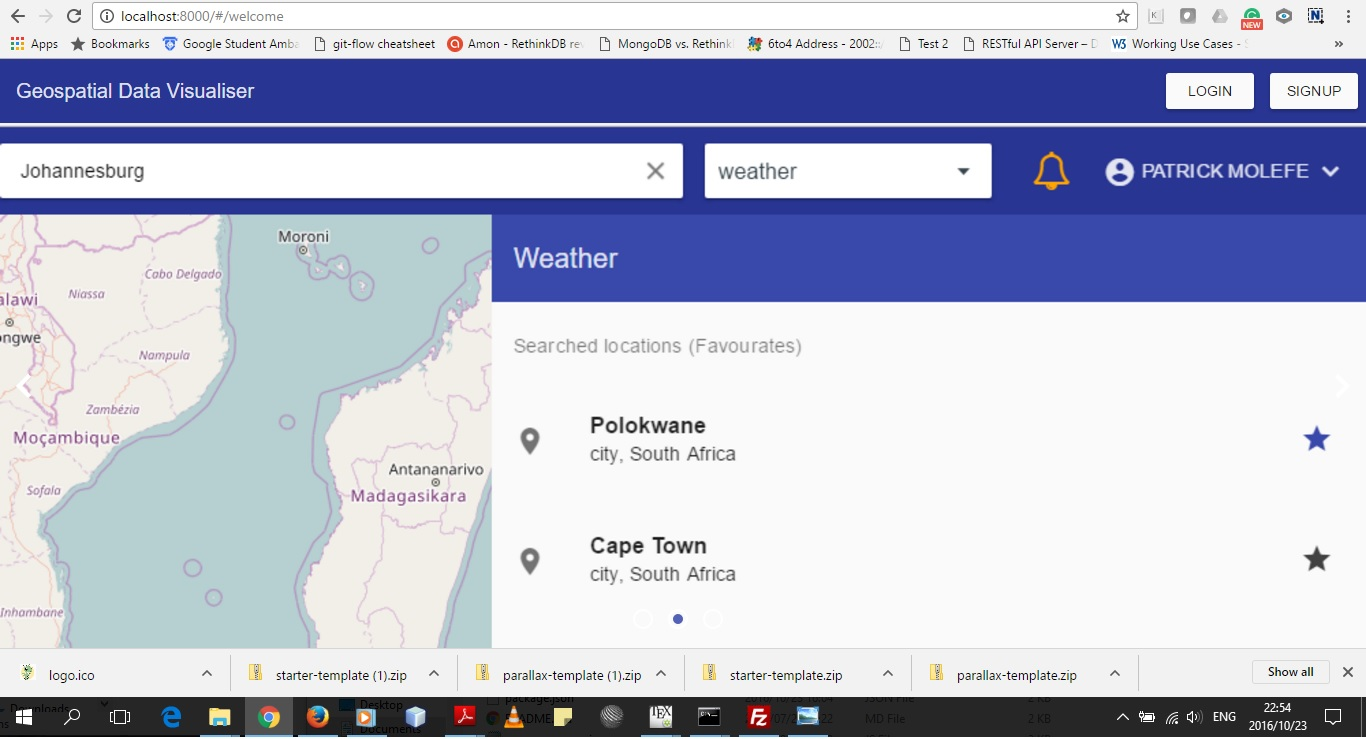
\includegraphics[width=\textwidth]{landingPage} \\[0.5cm]

\begin{enumerate}
	\item \textbf{Menu} 
	\item \textbf{Zoom Button} : With the zoom button feature, one may zoom, the map area, in and out. The "-" button is used for the function of zooming the map area out, and the "+" button is used for the function of zooming the map area in.
	\item \textbf{Map Area} : Display the map
	\item \textbf{Search Area} : Used to search for any location in the world
	\item \textbf{User menu} : The user menu is used to log the user in and out as well as check the settings. 
	\item \textbf{Center Navigation} : The Dropdown area is used to choose which functionality, of the site, you'd like to use. When loaded, the site lands on the weather center by default.
\end{enumerate}

\subsection{Features}
\subsubsection{Login}
\subsubsection{Registration}
\subsubsection{Location Search}
The search service, is used to search and load any place in the world. As shown in the figure below, you need to click in the search box and start typing the name of the place you are searching for. \\[0.5cm]
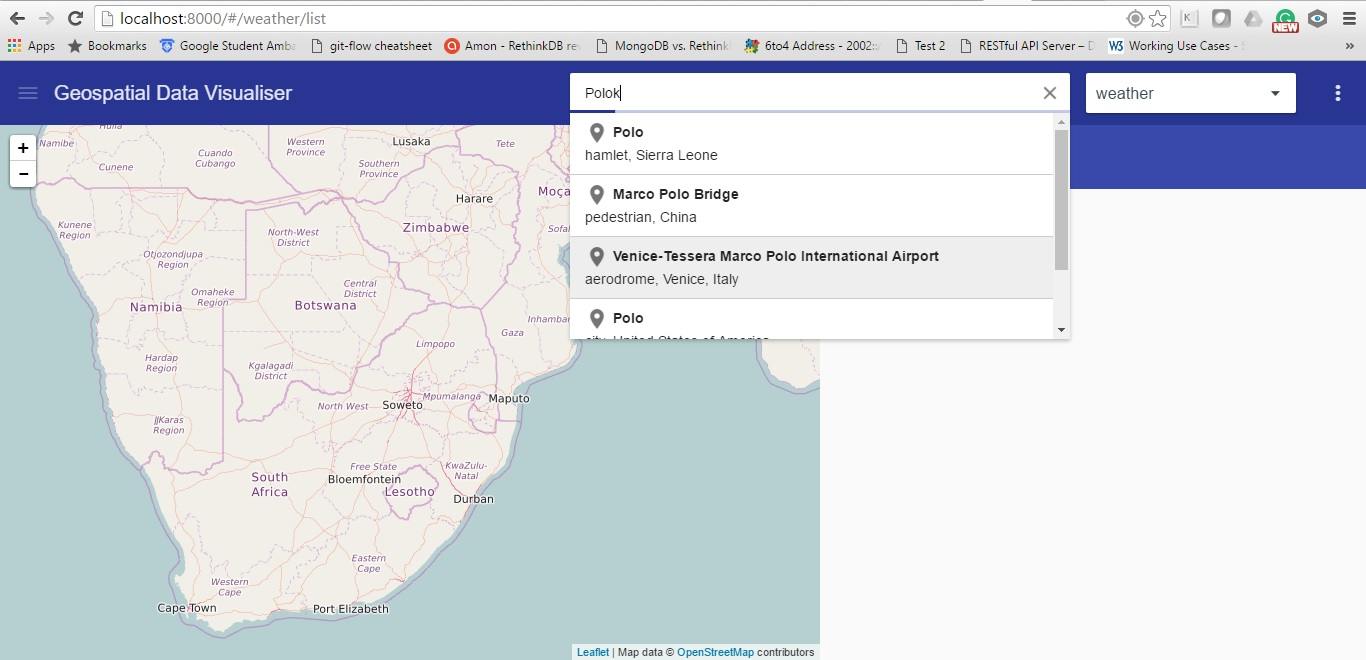
\includegraphics[width=\textwidth]{searchFunction} \\[0.5cm]
While searching a possible list of places will be loaded in a dropdown list as shown in the figure above. Once you have found the place you are looking for, use your mouse to point to the name of the place and click on that name, which will then activate a process of reloading the map to the place you have selected, like the figure shown below. A marker will be placed to show the location you queried. \\[0.5cm]
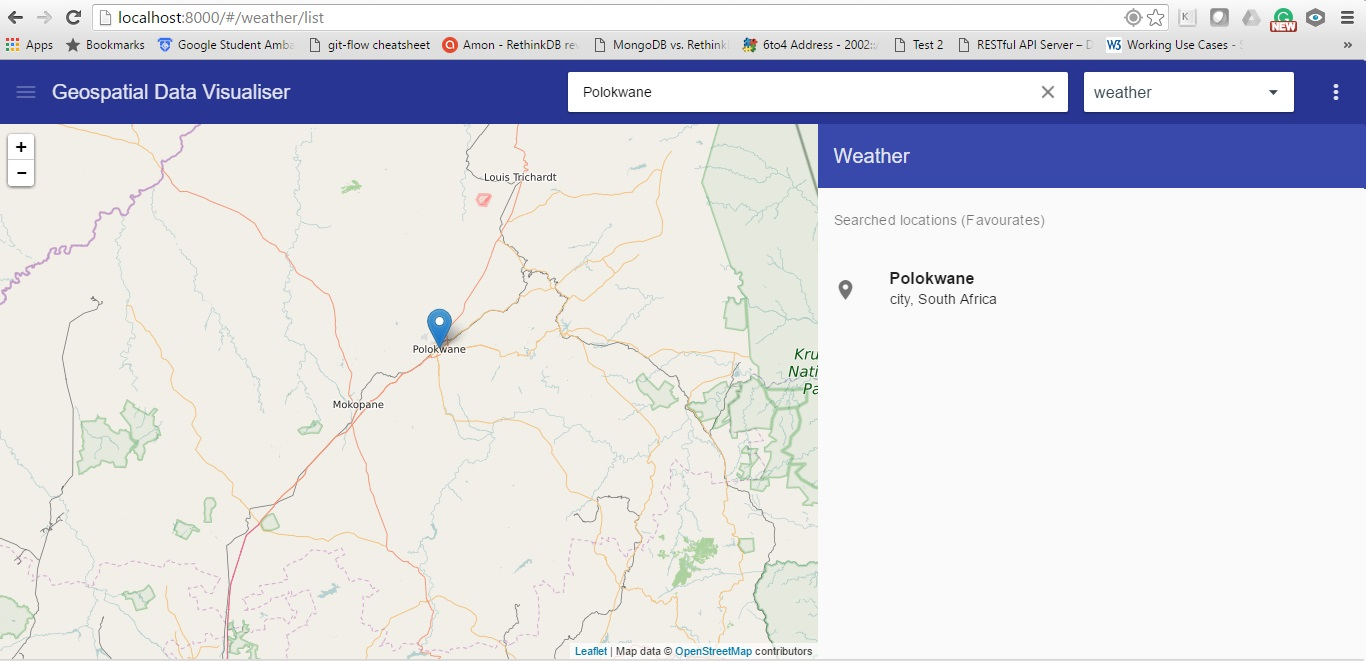
\includegraphics[width=\textwidth]{searchResult} \\[0.5cm]
The search feature is also linked to other functions of the site. When the weather center is currently active, the location name will be added to the listed of locations you have already searched for as shown above. These features will be explained in more detail in sections about the respective features.
\subsubsection{Disaster Center}
\subsubsection{Weather Center}
\subsubsection{Map Features}
		
	%-------------------------------------------------------------------------------------
	%		PART2
	%-------------------------------------------------------------------------------------
	
	\section{Part2: Setting up}
	\subsection{Installation}
This section will cover the configuration of the various servers on your platform. 
\subsubsection{Minimum Software Requirements}
To run the service you are required to have \href{https://git-scm.com}{git}, \href{https://nodejs.org}{NodeJS} v6 or higher (Which comes with \href{https://www.npmjs.com}{npm} v3 or higher), \href{https://www.rabbitmq.com/download.html}{RabbitMQ}, \href{https://www.mongodb.com/download-center?jmp=nav#community}{MongoDB} and \href{http://rethinkdb.com/docs/install}{RethinkDB} installed on your platform.
\subsubsection{Configuration}
	\begin{enumerate}
		\item \textbf{Download Source Code} \\
		The source code is located on \href{https://github.com}{Github} at the : \url{https://github.com/Coeus2016/geospatial-data-processor-and-visualizer}. You are required to clone the repository. There are two ways to clone the repository:\\
		\begin{itemize}
			\item By using the git command line. In the root folder run the following commands
			\begin{verbatim}
			$git clone https://github.com/Coeus2016/geospatial-data-processor-and
			-visualizer.git		
			\end{verbatim}
		
		\item By downloading the a *zip file from this url \url{https://github.com/Coeus2016/geospatial-data-processor-and-visualizer}\\
		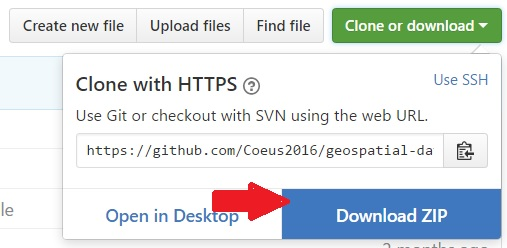
\includegraphics[width=\textwidth]{clone} \\[0.5cm]
		
		\end{itemize}
		
		\item \textbf{Installing Required Modules}\\
		Now that you have downloaded the repository, navigate to the root folder and perform the following commands.
		\begin{verbatim}
			$git submodule update --init --recursive
			$npm install			
			\end{verbatim}
			These commands updated the submodules and install the node modules required to run the server	
	\end{enumerate}

\subsubsection{Starting The Service}
Once you have downloaded and installed all required modules, you are ready to start the service. The following steps need to be followed to insure a safe start of the system.
\begin{enumerate}
	\item Before you can start the application server, you need to make sure all other used services (RethinkDB, MongoDB, RabbitMQ) have been started\footnote{A lot of the time they are configured to start when the computer is booted otherwise you are required to start the services manually in different terminal windows.}. 
	\item Once the other services have been started, running the following command will start the application. 
	\begin{verbatim}
		$npm start			
	\end{verbatim}
	The backend Server will run on port 3200, the scrapper on port 3500 and the webserver on port 3000. To view the website, simply visit \url{http://localhost:3000} on your browser.
\end{enumerate}
\subsection{Code Maintenance}
	
	
	%-------------------------------------------------------------------------------------
	%		REFERENCES
	%-------------------------------------------------------------------------------------
	
	\section{References}
	\bibliography{references}
	
	\end{document}
